\section{Results}

The systemwas implemented as described in the previous sections.
We tested the system by applyind a step function of 1.89 N, and recording the system response.
The resulting magnet position can be seen in Figure \ref{fig:position}.

\begin{figure}[h]
    \centering
    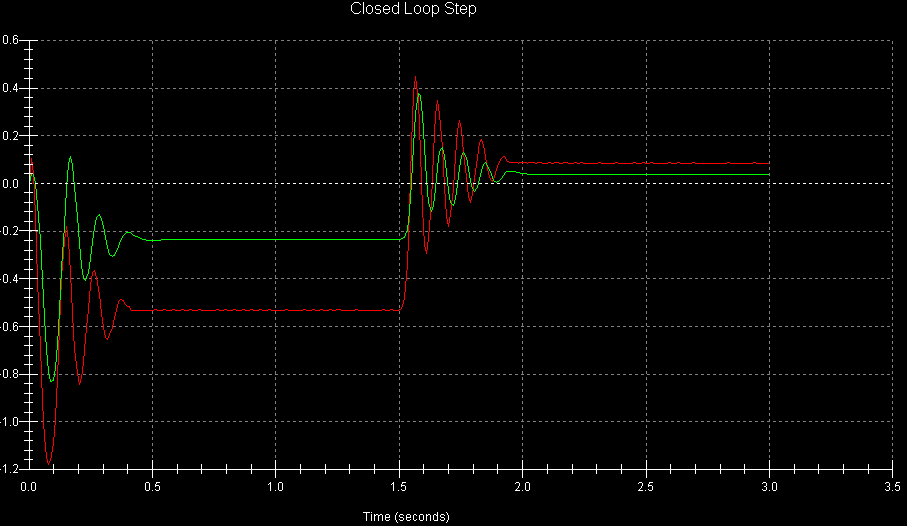
\includegraphics[width=1\textwidth]{position}
    \caption{System Response: Position}
    \label{fig:position}
\end{figure}

The magnet velocity is shown in Figure \ref{fig:velocity}.

\begin{figure}[h]
    \centering
    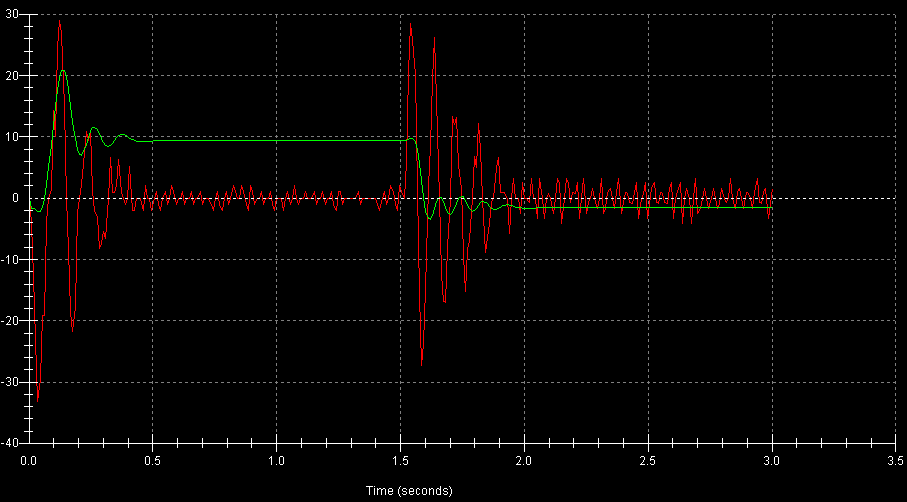
\includegraphics[width=1\textwidth]{velocity}
    \caption{System Response: Velocity}
    \label{fig:velocity}
\end{figure}


%some equations....
\begin{equation}
	\label{eq:settling_time}
	T_{s} = {\frac {y}{\zeta \, \omega_n}}
\end{equation}

\begin{equation}
	\label{eq:overshoot}
	\zeta = -{\frac {ln{OS}}{\sqrt{{\pi}^{2}+{ln{OS}}^{2}}}}
\end{equation}
